


\if0
\begin{table*}[h]
\centering
\tiny
\resizebox{1.0\linewidth}{!}{
\begin{tabular}{l|cl|cl|cl|cc}
\hline
                       & \multicolumn{2}{c|}{\textbf{In-domain accuracy}}                & \multicolumn{2}{c|}{\textbf{OOS recall}}                        & \multicolumn{2}{c|}{\textbf{OOS precision}}                     & \multicolumn{2}{c}{\textbf{OOS F1}}              \\
                       & \textbf{5-shot}         & \multicolumn{1}{c|}{\textbf{10-shot}} & \textbf{5-shot}         & \multicolumn{1}{c|}{\textbf{10-shot}} & \textbf{5-shot}         & \multicolumn{1}{c|}{\textbf{10-shot}} & \textbf{5-shot}                      & \textbf{10-shot} \\ \cline{2-9} 
classifier             & 77.7 $\pm$ 0.6          & 83.2 $\pm$ 0.6                        & \textbf{91.9 $\pm$ 1.1}          & \textbf{92.9 $\pm$ 0.8}               & 53.9 $\pm$ 0.8          & 58.2 $\pm$ 1.0                        & 68.0 $\pm$ 1.0          &      71.6 $\pm$ 0.8            \\
DNNC          & \textbf{84.9 $\pm$ 0.8} & \textbf{91.6 $\pm$ 0.3}               & 90.1 $\pm$ 1.6 & 83.0 $\pm$ 2.0                        & \textbf{64.7 $\pm$ 2.5} & \textbf{81.4 $\pm$ 2.0}               &  \textbf{75.3 $\pm$ 2.0}        &   \textbf{82.1 $\pm$ 0.3}               \\ \hdashline
classifier (full-shot) & \multicolumn{2}{c|}{92.9 $\pm$ 0.2}                & \multicolumn{2}{c|}{90.2 $\pm$ 0.5}                & \multicolumn{2}{c|}{76.7 $\pm$ 0.7}                & \multicolumn{2}{c}{82.9 $\pm$ 0.6}         \\ \hline
\end{tabular}}\caption{Testing results on the whole dataset (5 runs).}
\label{table:wholeDataset}
%\vspace{-1em}
\end{table*}
\fi

%%%%%%%%%%%%%%%%%%%%%%%%%%%%%%%%%%%%%%%%%%%%%%%%%%
% \begin{table*}[]
% \centering
% \tiny
% \resizebox{0.8\linewidth}{!}{
% \begin{tabular}{lcccccc}
% \hline
% \multicolumn{1}{l|}{}                 & \multicolumn{2}{c|}{\textbf{In-domain accuracy}}                                                     & \multicolumn{2}{c|}{\textbf{OOS recall}}                                                    & \multicolumn{2}{c}{\textbf{OOS precision}}                               \\
% \multicolumn{1}{l|}{\textbf{5-Shot}}  & \textbf{Banking}                       & \multicolumn{1}{c|}{\textbf{Credit cards}}                 & \textbf{Banking}                       & \multicolumn{1}{c|}{\textbf{Credit cards}}                 & \textbf{Banking}                       & \textbf{Credit cards}                 \\ \hline
% \multicolumn{1}{l|}{classifier}       & 79.7 $\pm$ 1.8          & \multicolumn{1}{c|}{79.9 $\pm$ 3.7}          & 93.3 $\pm$ 2.9          & \multicolumn{1}{c|}{93.3 $\pm$ 3.0}          & 92.5  $\pm$ 0.9         & 93.6 $\pm$ 1.3          \\
% \multicolumn{1}{l|}{classifier-EDA}   & 79.9 $\pm$ 3.0          & \multicolumn{1}{c|}{73.1 $\pm$ 5.0}          & 91.0 $\pm$ 2.6          & \multicolumn{1}{c|}{94.1  $\pm$ 2.6}         & 92.6  $\pm$ 1.5         & 90.0 $\pm$ 1.7          \\
% \multicolumn{1}{l|}{classifier-BT}    & 77.2  $\pm$ 2.8         & \multicolumn{1}{c|}{70.3 $\pm$ 4.4}          & 91.5 $\pm$ 2.4          & \multicolumn{1}{c|}{91.1 $\pm$ 1.8}          & 91.4 $\pm$ 1.2          & 89.5 $\pm$ 1.8          \\
% \multicolumn{1}{l|}{nli-Scratch}      & 83.4 $\pm$ 1.9          & \multicolumn{1}{c|}{84.6 $\pm$ 3.2}          & 93.2 $\pm$ 2.7          & \multicolumn{1}{c|}{96.4 $\pm$ 1.0}          & 96.2 $\pm$ 0.9          & 95.9 $\pm$ 1.1          \\
% \multicolumn{1}{l|}{nli-Fine-Tune}    & \textbf{88.6 $\pm$ 1.3} & \multicolumn{1}{c|}{\textbf{90.5 $\pm$ 2.9}} & \textbf{94.7 $\pm$ 1.0} & \multicolumn{1}{c|}{\textbf{97.7 $\pm$ 1.1}} & \textbf{97.0 $\pm$ 0.3} & \textbf{97.8 $\pm$ 0.5} \\ \hline
%                                     %   & \multicolumn{1}{l}{}                   & \multicolumn{1}{l}{}                                        & \multicolumn{1}{l}{}                   & \multicolumn{1}{l}{}                                        & \multicolumn{1}{l}{}                   & \multicolumn{1}{l}{}                   \\ \hline
% \multicolumn{1}{l|}{\textbf{5-Shot}}  & \textbf{Work}                          & \multicolumn{1}{c|}{\textbf{Travel}}                        & \textbf{Work}                          & \multicolumn{1}{c|}{\textbf{Travel}}                        & \textbf{Work}                          & \textbf{Travel}                        \\ \hline
% \multicolumn{1}{l|}{classifier}       & 84.4 $\pm$ 1.9          & \multicolumn{1}{c|}{87.8 $\pm$ 2.5}          & 94.8 $\pm$ 1.6          & \multicolumn{1}{c|}{96.1 $\pm$ 0.9}          & 95.4 $\pm$ 0.7         & 94.7 $\pm$ 1.0          \\
% \multicolumn{1}{l|}{classifier-EDA}   & 80.5 $\pm$ 3.3          & \multicolumn{1}{c|}{88.2 $\pm$ 2.4}          & 95.2 $\pm$ 1.6          & \multicolumn{1}{c|}{94.6 $\pm$ 2.1}          & 92.8 $\pm$ 1.3         & 94.9 $\pm$ 1.0          \\
% \multicolumn{1}{l|}{classifier-BT}    & 80.3 $\pm$ 3.4          & \multicolumn{1}{c|}{90.8 $\pm$ 2.4}          & 94.4 $\pm$ 1.1          & \multicolumn{1}{c|}{92.3 $\pm$ 1.9}          & 93.1 $\pm$ 1.0         & 95.9 $\pm$ 1.1          \\
% \multicolumn{1}{l|}{nli-Scratch}      & 83.2 $\pm$ 2.1          & \multicolumn{1}{c|}{87.8 $\pm$ 3.5}          & 96.3 $\pm$ 1.7          & \multicolumn{1}{c|}{94.9 $\pm$ 2.8}          & 96.7 $\pm$ 0.9          & 94.9 $\pm$ 1.4          \\
% \multicolumn{1}{l|}{nli-Fine-Tune}    & \textbf{89.9 $\pm$ 3.2} & \multicolumn{1}{c|}{\textbf{91.8 $\pm$ 1.6}} & \textbf{96.7 $\pm$ 1.1} & \multicolumn{1}{c|}{\textbf{96.4 $\pm$ 1.2}} & \textbf{97.9 $\pm$ 1.1} & \textbf{96.5 $\pm$ 0.7} \\ \hline
%                                     %   & \multicolumn{1}{l}{}                   & \multicolumn{1}{l}{}                                        & \multicolumn{1}{l}{}                   & \multicolumn{1}{l}{}                                        & \multicolumn{1}{l}{}                   & \multicolumn{1}{l}{}                   \\
%                                       & \multicolumn{1}{l}{}                   & \multicolumn{1}{l}{}                                        & \multicolumn{1}{l}{}                   & \multicolumn{1}{l}{}                                        & \multicolumn{1}{l}{}                   & \multicolumn{1}{l}{}                   \\ \hline
% \multicolumn{1}{l|}{}                 & \multicolumn{2}{c|}{\textbf{In-domain accuracy}}                                                     & \multicolumn{2}{c|}{\textbf{OOS recall}}                                                    & \multicolumn{2}{c}{\textbf{OOS precision}}                             \\
% \multicolumn{1}{l|}{\textbf{10-Shot}} & \textbf{Banking}                       & \multicolumn{1}{c|}{\textbf{Credit cards}}                 & \textbf{Banking}                       & \multicolumn{1}{c|}{\textbf{Credit cards}}                 & \textbf{Banking}                       & \textbf{Credit cards}                 \\ \hline
% \multicolumn{1}{l|}{classifier}       & 85.2 $\pm$ 1.3          & \multicolumn{1}{c|}{83.7 $\pm$ 2.1}          & 93.3 $\pm$ 1.0          & \multicolumn{1}{c|}{93.8 $\pm$ 1.4}          & 94.4 $\pm$ 0.5          & 93.9 $\pm$ 0.9          \\
% \multicolumn{1}{l|}{classifier-EDA}   & 82.5 $\pm$ 1.3         & \multicolumn{1}{c|}{79.3 $\pm$ 1.7}          & \textbf{95.9 $\pm$ 0.8}          & \multicolumn{1}{c|}{96.8 $\pm$ 0.8}          & 93.3 $\pm$ 0.4         & 92.3 $\pm$ 0.8          \\
% \multicolumn{1}{l|}{classifier-BT}    & 82.2 $\pm$ 1.9          & \multicolumn{1}{c|}{82.9 $\pm$ 1.8}          & 94.9 $\pm$ 1.9 & \multicolumn{1}{c|}{89.3 $\pm$ 2.0}          & 93.1 $\pm$ 0.8          & 94.3 $\pm$ 0.6         \\
% \multicolumn{1}{l|}{nli-Scratch}      & 89.6 $\pm$ 1.6          & \multicolumn{1}{c|}{92.1 $\pm$ 1.1}          & 92.1 $\pm$ 3.1          & \multicolumn{1}{c|}{94.8 $\pm$ 1.2}          & 97.5 $\pm$ 0.9 & \textbf{98.1 $\pm$ 0.4} \\
% \multicolumn{1}{l|}{nli-Fine-Tune}    & \textbf{91.2 $\pm$ 1.1} & \multicolumn{1}{c|}{\textbf{92.1 $\pm$ 1.0}} & 94.8 $\pm$ 1.1          & \multicolumn{1}{c|}{\textbf{97.8 $\pm$ 0.8}} & \textbf{97.5 $\pm$ 0.4}          & 97.8 $\pm$ 0.3         \\ \hline
%                                     %   &                                        &                                                             &                                        &                                                             &                                        &                                        \\ \hline
% \multicolumn{1}{l|}{\textbf{10-Shot}} & \textbf{Work}                          & \multicolumn{1}{c|}{\textbf{Travel}}                        & \textbf{Work}                          & \multicolumn{1}{c|}{\textbf{Travel}}                        & \textbf{Work}                          & \textbf{Travel}                        \\ \hline
% \multicolumn{1}{l|}{classifier}       & 86.0 $\pm$ 2.2          & \multicolumn{1}{c|}{93.0 $\pm$ 1.2}          & 97.2 $\pm$ 0.7          & \multicolumn{1}{c|}{94.8 $\pm$ 0.9}          & 94.5 $\pm$ 0.8         & 96.8 $\pm$ 0.6          \\
% \multicolumn{1}{l|}{classifier-EDA}   & 86.4 $\pm$ 1.7          & \multicolumn{1}{c|}{93.0 $\pm$ 1.0}          & 97.0 $\pm$ 0.9          & \multicolumn{1}{c|}{95.2 $\pm$ 1.3}          & 94.7 $\pm$ 0.7          & 96.9 $\pm$ 0.5         \\
% \multicolumn{1}{l|}{classifier-BT}    & 83.7 $\pm$ 1.7          & \multicolumn{1}{c|}{91.9 $\pm$ 1.1}          & \textbf{97.4 $\pm$ 0.9} & \multicolumn{1}{c|}{\textbf{96.1 $\pm$ 0.8}} & 93.6 $\pm$ 0.7         & 96.4 $\pm$ 0.5          \\
% \multicolumn{1}{l|}{nli-Scratch}      & 92.6 $\pm$ 1.7          & \multicolumn{1}{c|}{\textbf{96.4 $\pm$ 0.6}} & 94.1 $\pm$ 1.4         & \multicolumn{1}{c|}{84.8 $\pm$ 3.0}          & 98.4 $\pm$ 0.6          & \textbf{98.5 $\pm$ 0.3} \\
% \multicolumn{1}{l|}{nli-Fine-Tune}    & \textbf{95.0 $\pm$ 1.0} & \multicolumn{1}{c|}{96.0 $\pm$ 0.8}          & 95.5 $\pm$ 0.9          & \multicolumn{1}{c|}{93.3 $\pm$ 1.9}          & \textbf{99.0 $\pm$ 0.4} & 98.3 $\pm$ 0.4          \\ \hline
% \end{tabular}}\caption{Testing results on the four different domains.}
% \label{table:fourDomain}
% \end{table*}
%%%%%%%%%%%%%%%%%%%%%%%%%%%%%%%%%%%%%%%%%%%%%%%%%%


\section{Experimental Results}

This section shows our experimental results.
Appendix~\ref{extra-results} shows some additional figures.

\subsection{Model Performance CLINC150 Dataset}
\paragraph{Single domains}
We first show test set results of 5-shot and 10-shot in-domain classification and OOS detection accuracy in Table~\ref{table:fourDomain} for the four selected domains.
In the 5-shot setting, the proposed DNNC method consistently attains the best results across all the four domains.
The comparison between DNNC-scratch and DNNC shows that our NLI task transfer is effective.
In the 10-shot setting, all the approaches generally experience an accuracy improvement due to the additional training data, and the dominant performance of DNNC weakens, although it remains highly competitive.
We can see that our DNNC is comparable with or even surpasses some of the 50-shot classifier's scores, and the data augmentation techniques are not always helpful when we use the strong pre-trained model.





\paragraph{Entire CLINC150 dataset}
Next, Table~\ref{table:wholeDataset} shows results to compare our method with the classifier and USE+ConveRT baselines, on the entire CLINC150 dataset with the 150 intents. USE+ConveRT performs worse than the RoBERTa-based classifier on the OOD detection task. 
The advantage of DNNC for in-domain intent detection is clear, with its 10-shot in-domain accuracy close to the upper-bound accuracy for the classifier baseline.
One observation is that our DNNC method tends to be more confident about its prediction, with the increasing number of the training examples; as a result, the OOS recall becomes lower in the 10-shot setting, while the OOS precision is much higher than the other baselines.
Better controlling the confidence output of the model is an interesting direction for future work.

When the USE+ConveRT baseline is evaluated along with the OOS detection task, its overall accuracy is not as good as the other RoBERTa-based models, despite its potential in the purely in-domain classification.
This indicates that the fine-tuned (Ro)BERT(a) models are more robust to out-of-distribution examples than shallower models like USE+ConveRT, also suggested in \citet{acl-ood}.
%\textcolor{red}{Furthermore, DNNC method outperforms or stays competitive with the classifier on the OOS detection task. [Reviewer2: this is not supported by OOS recall column in Table 4.]}

%%%%%%%%%%%%%%%%%%%%%%%%%%%%%%%%%%%%%%%%%%%%%%%%%%
\if0
\begin{table*}[t]
\centering
\small
\resizebox{1.0\linewidth}{!}{
\begin{tabular}{l|cl|cl|cl|cc}
\hline
                       & \multicolumn{2}{c|}{\textbf{In-domain accuracy}}                & \multicolumn{2}{c|}{\textbf{OOS recall}}                        & \multicolumn{2}{c|}{\textbf{OOS precision}}                     & \multicolumn{2}{c}{\textbf{OOS F1}}              \\
                       & \textbf{5-shot}         & \multicolumn{1}{c|}{\textbf{10-shot}} & \textbf{5-shot}         & \multicolumn{1}{c|}{\textbf{10-shot}} & \textbf{5-shot}         & \multicolumn{1}{c|}{\textbf{10-shot}} & \textbf{5-shot}                      & \textbf{10-shot} \\ \cline{2-9} 
classifier             & 77.7 $\pm$ 0.6          & 83.2 $\pm$ 0.6                        & \textbf{91.9 $\pm$ 1.1}          & \textbf{92.9 $\pm$ 0.8}               & 53.9 $\pm$ 0.8          & 58.2 $\pm$ 1.0                        & 68.0 $\pm$ 1.0          &      71.6 $\pm$ 0.8            \\
DNNC          & \textbf{84.9 $\pm$ 0.8} & \textbf{91.6 $\pm$ 0.3}               & 90.1 $\pm$ 1.6 & 83.0 $\pm$ 2.0                        & \textbf{64.7 $\pm$ 2.5} & \textbf{81.4 $\pm$ 2.0}               &  \textbf{75.3 $\pm$ 2.0}        &   \textbf{82.1 $\pm$ 0.3}               \\ \hdashline
classifier (full-shot) & \multicolumn{2}{c|}{92.9 $\pm$ 0.2}                & \multicolumn{2}{c|}{90.2 $\pm$ 0.5}                & \multicolumn{2}{c|}{76.7 $\pm$ 0.7}                & \multicolumn{2}{c}{82.9 $\pm$ 0.6}         \\ \hline
\end{tabular}}\caption{Testing results on the whole dataset.}
\label{table:wholeDataset}
%\vspace{-1em}
\end{table*}
\fi


%%%%%%%%%%%%%%%%%%%%%%%%%%%%%%%%%%%
\begin{figure*}[t!]%bp]
\centering
\begin{minipage}[t]{1.0\textwidth}
    \centering
    %\begin{center}
    %\includegraphics[width=1.0\linewidth]{./images/5-10-shot-Conf-flat.png}
    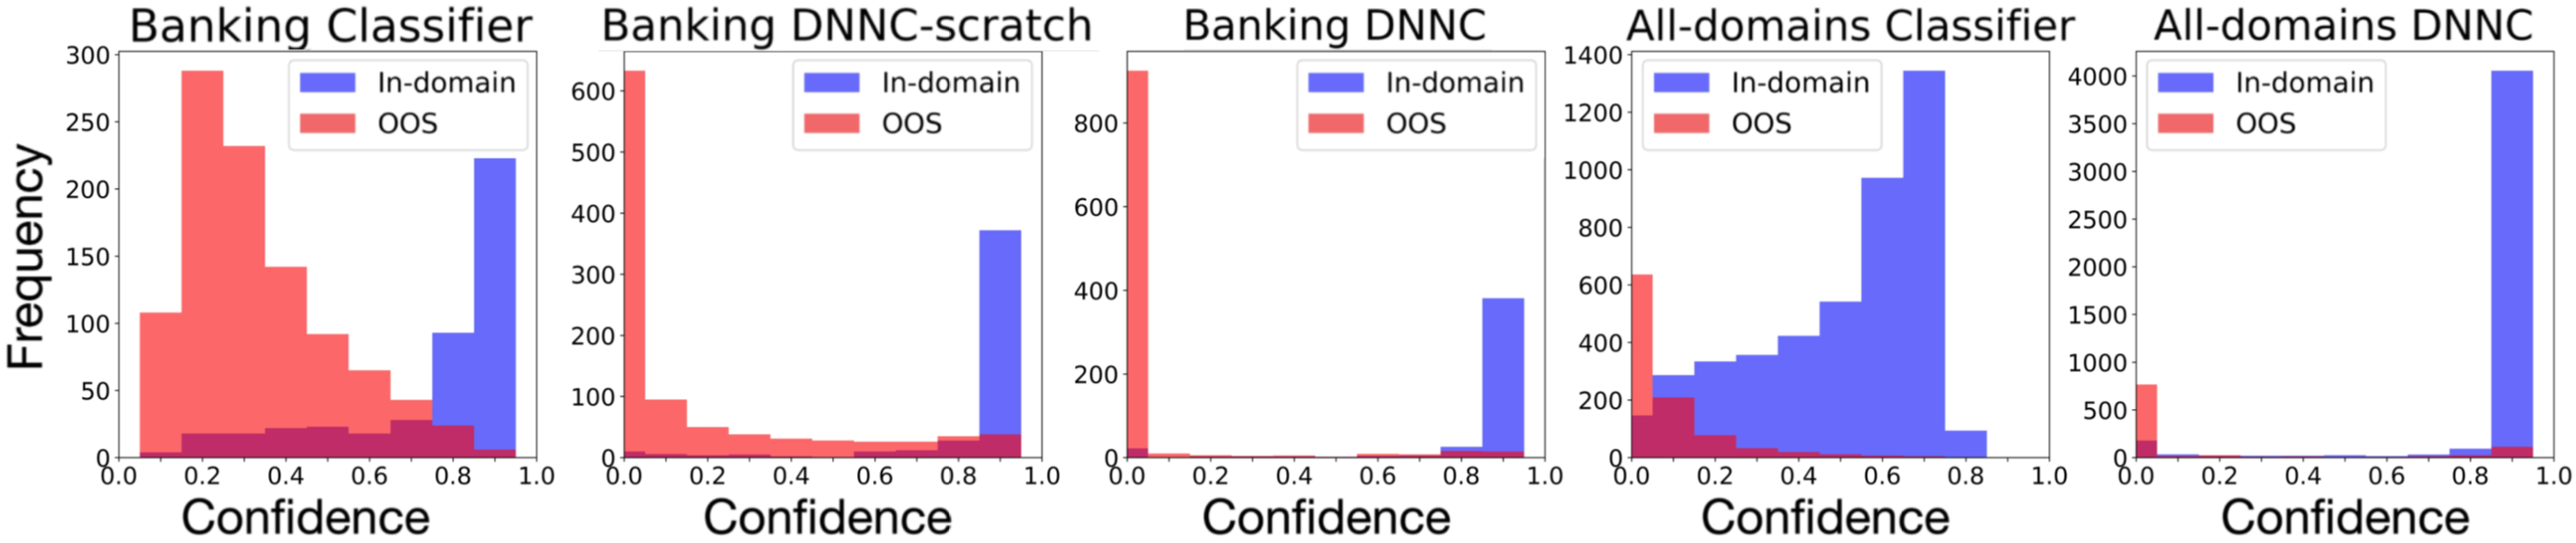
\includegraphics[width=0.92\linewidth]{./images/conf_hist_main.png}
    % \end{center}
    \caption{Model confidence level on 5-shot test sets for the banking domain and all domains.}
    \label{fig:separation}
\end{minipage}%

\vspace{10pt}

%\subfigure[]{
\begin{minipage}[t]{0.71\textwidth}
    \centering
    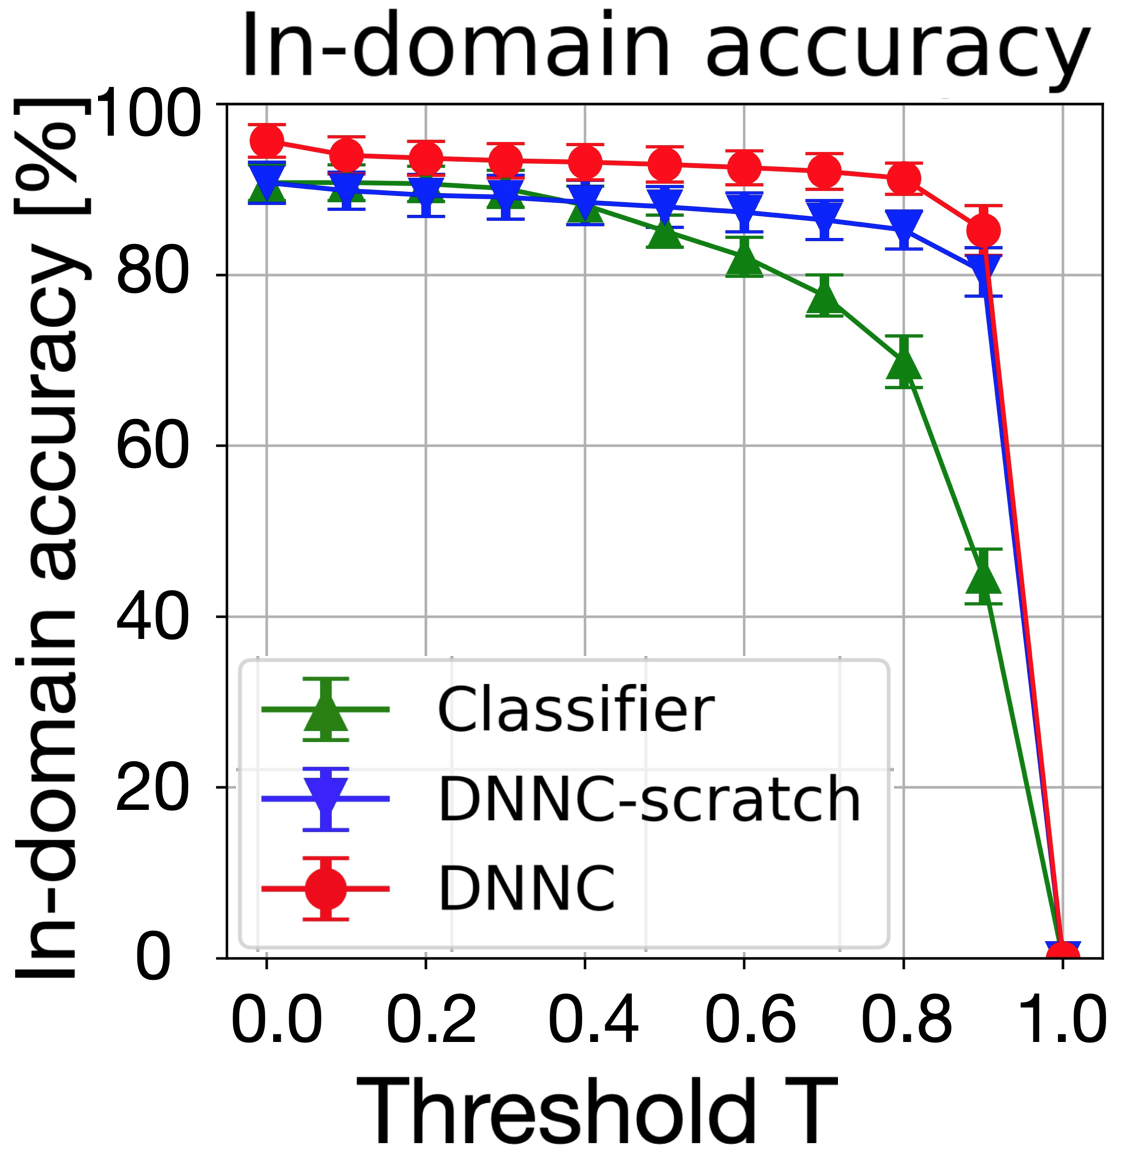
\includegraphics[width=0.3\linewidth]{./images/curve_main_in_acc.png}
    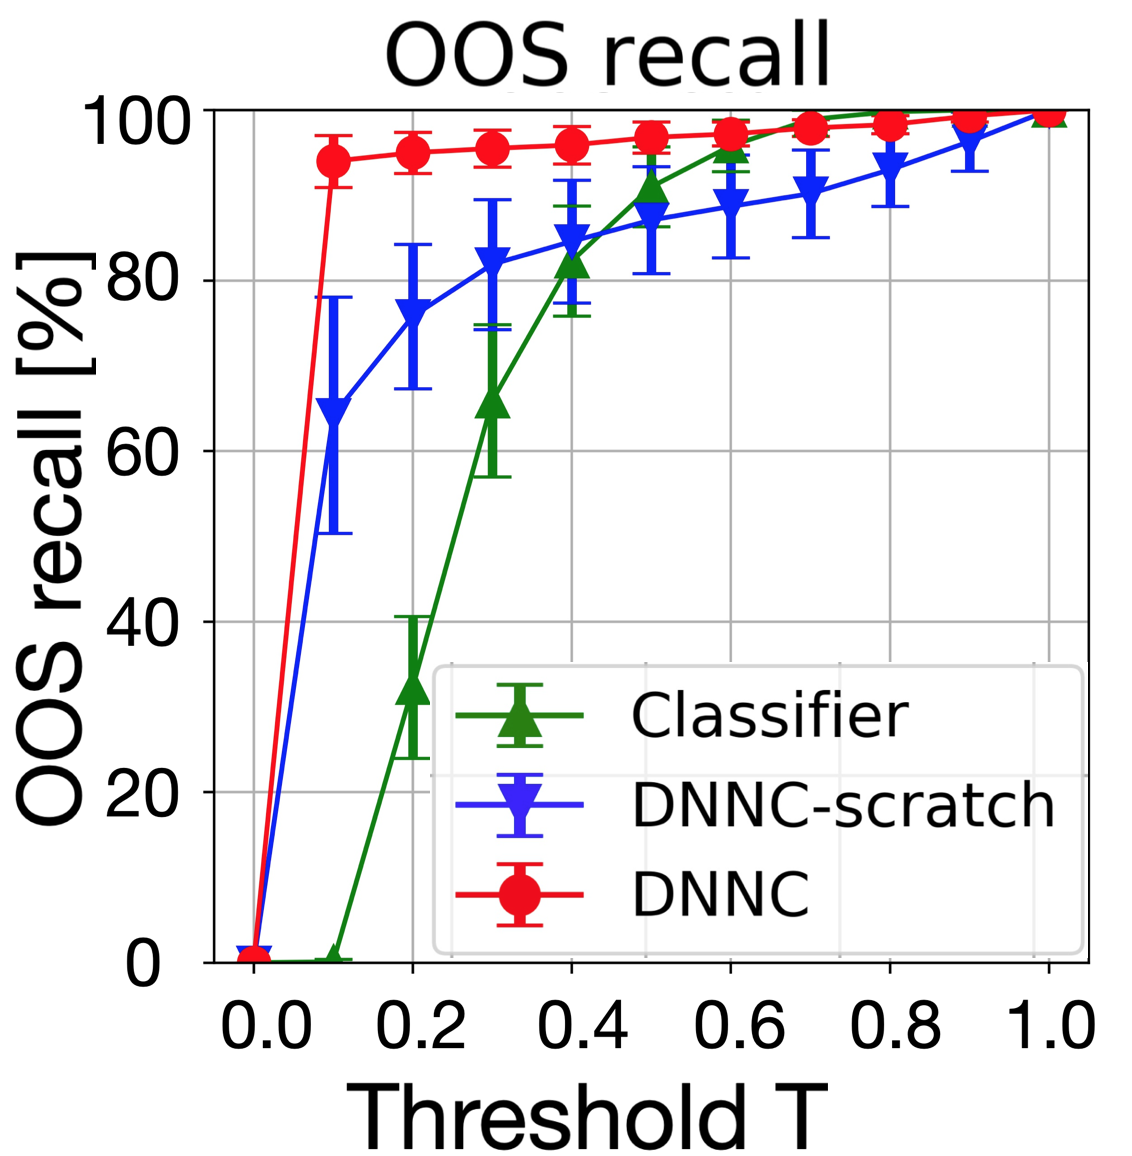
\includegraphics[width=0.3\linewidth]{./images/curve_main_oos_recall.png}
    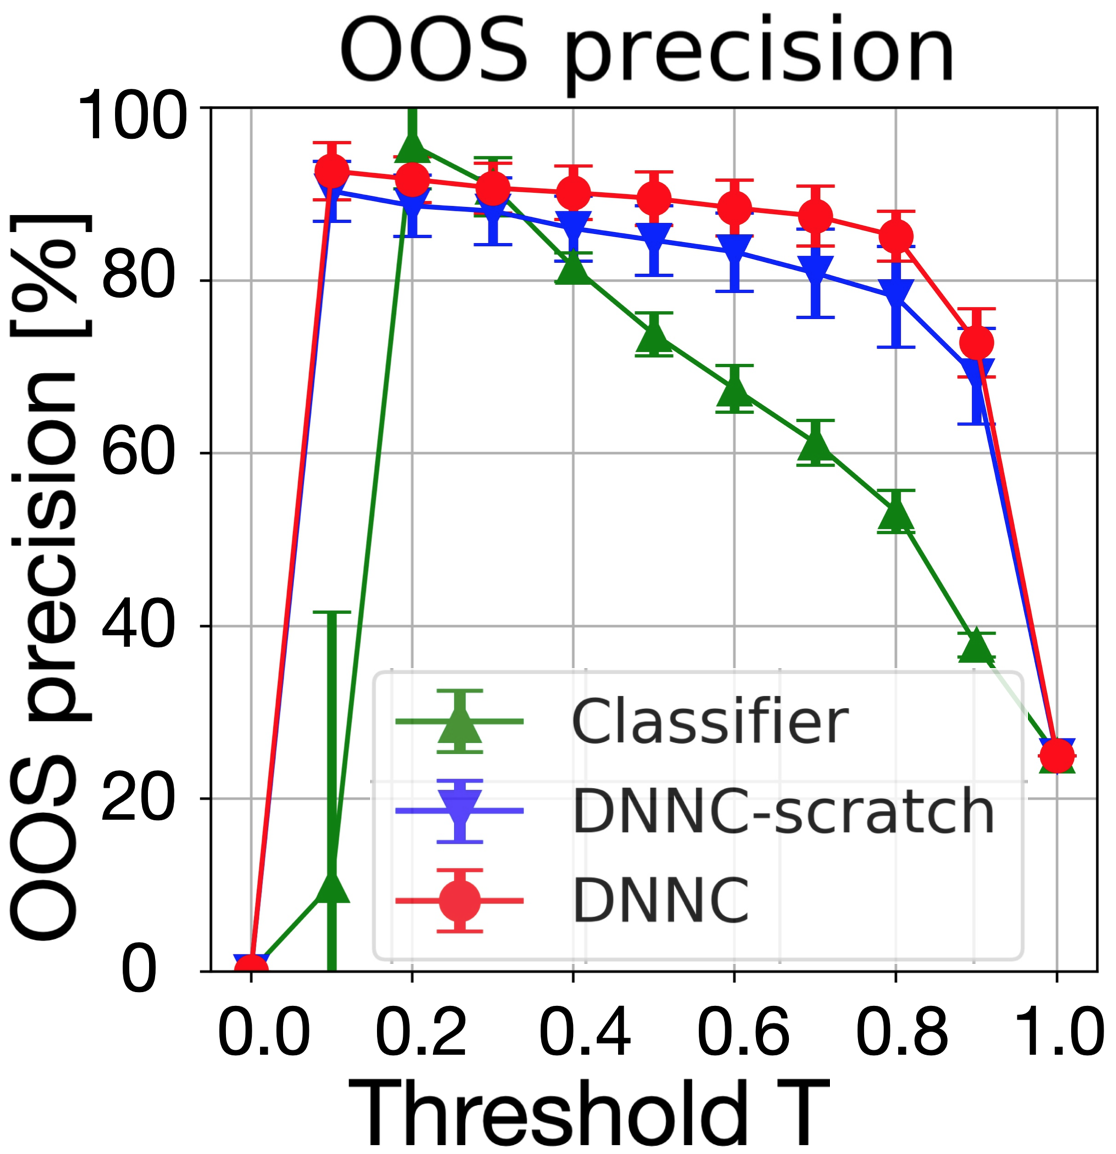
\includegraphics[width=0.3\linewidth]{./images/curve_main_oos_prec.png}
    % \includegraphics[width=0.325\linewidth]{./images/La}
    \caption{Development set results on the banking domain in the 5-shot setting. In this series of plots, a model with a higher area-under-the-curve is more robust.}
    \label{fig:robust}
    \end{minipage}%
\hfill
%}%
%\subfigure[]{
\begin{minipage}[t]{0.25\textwidth}
    \centering
    % \includegraphics[width=1.651in]{FMeasures/FBMS_Score.eps}\\
    % \vspace{0.02cm}
    %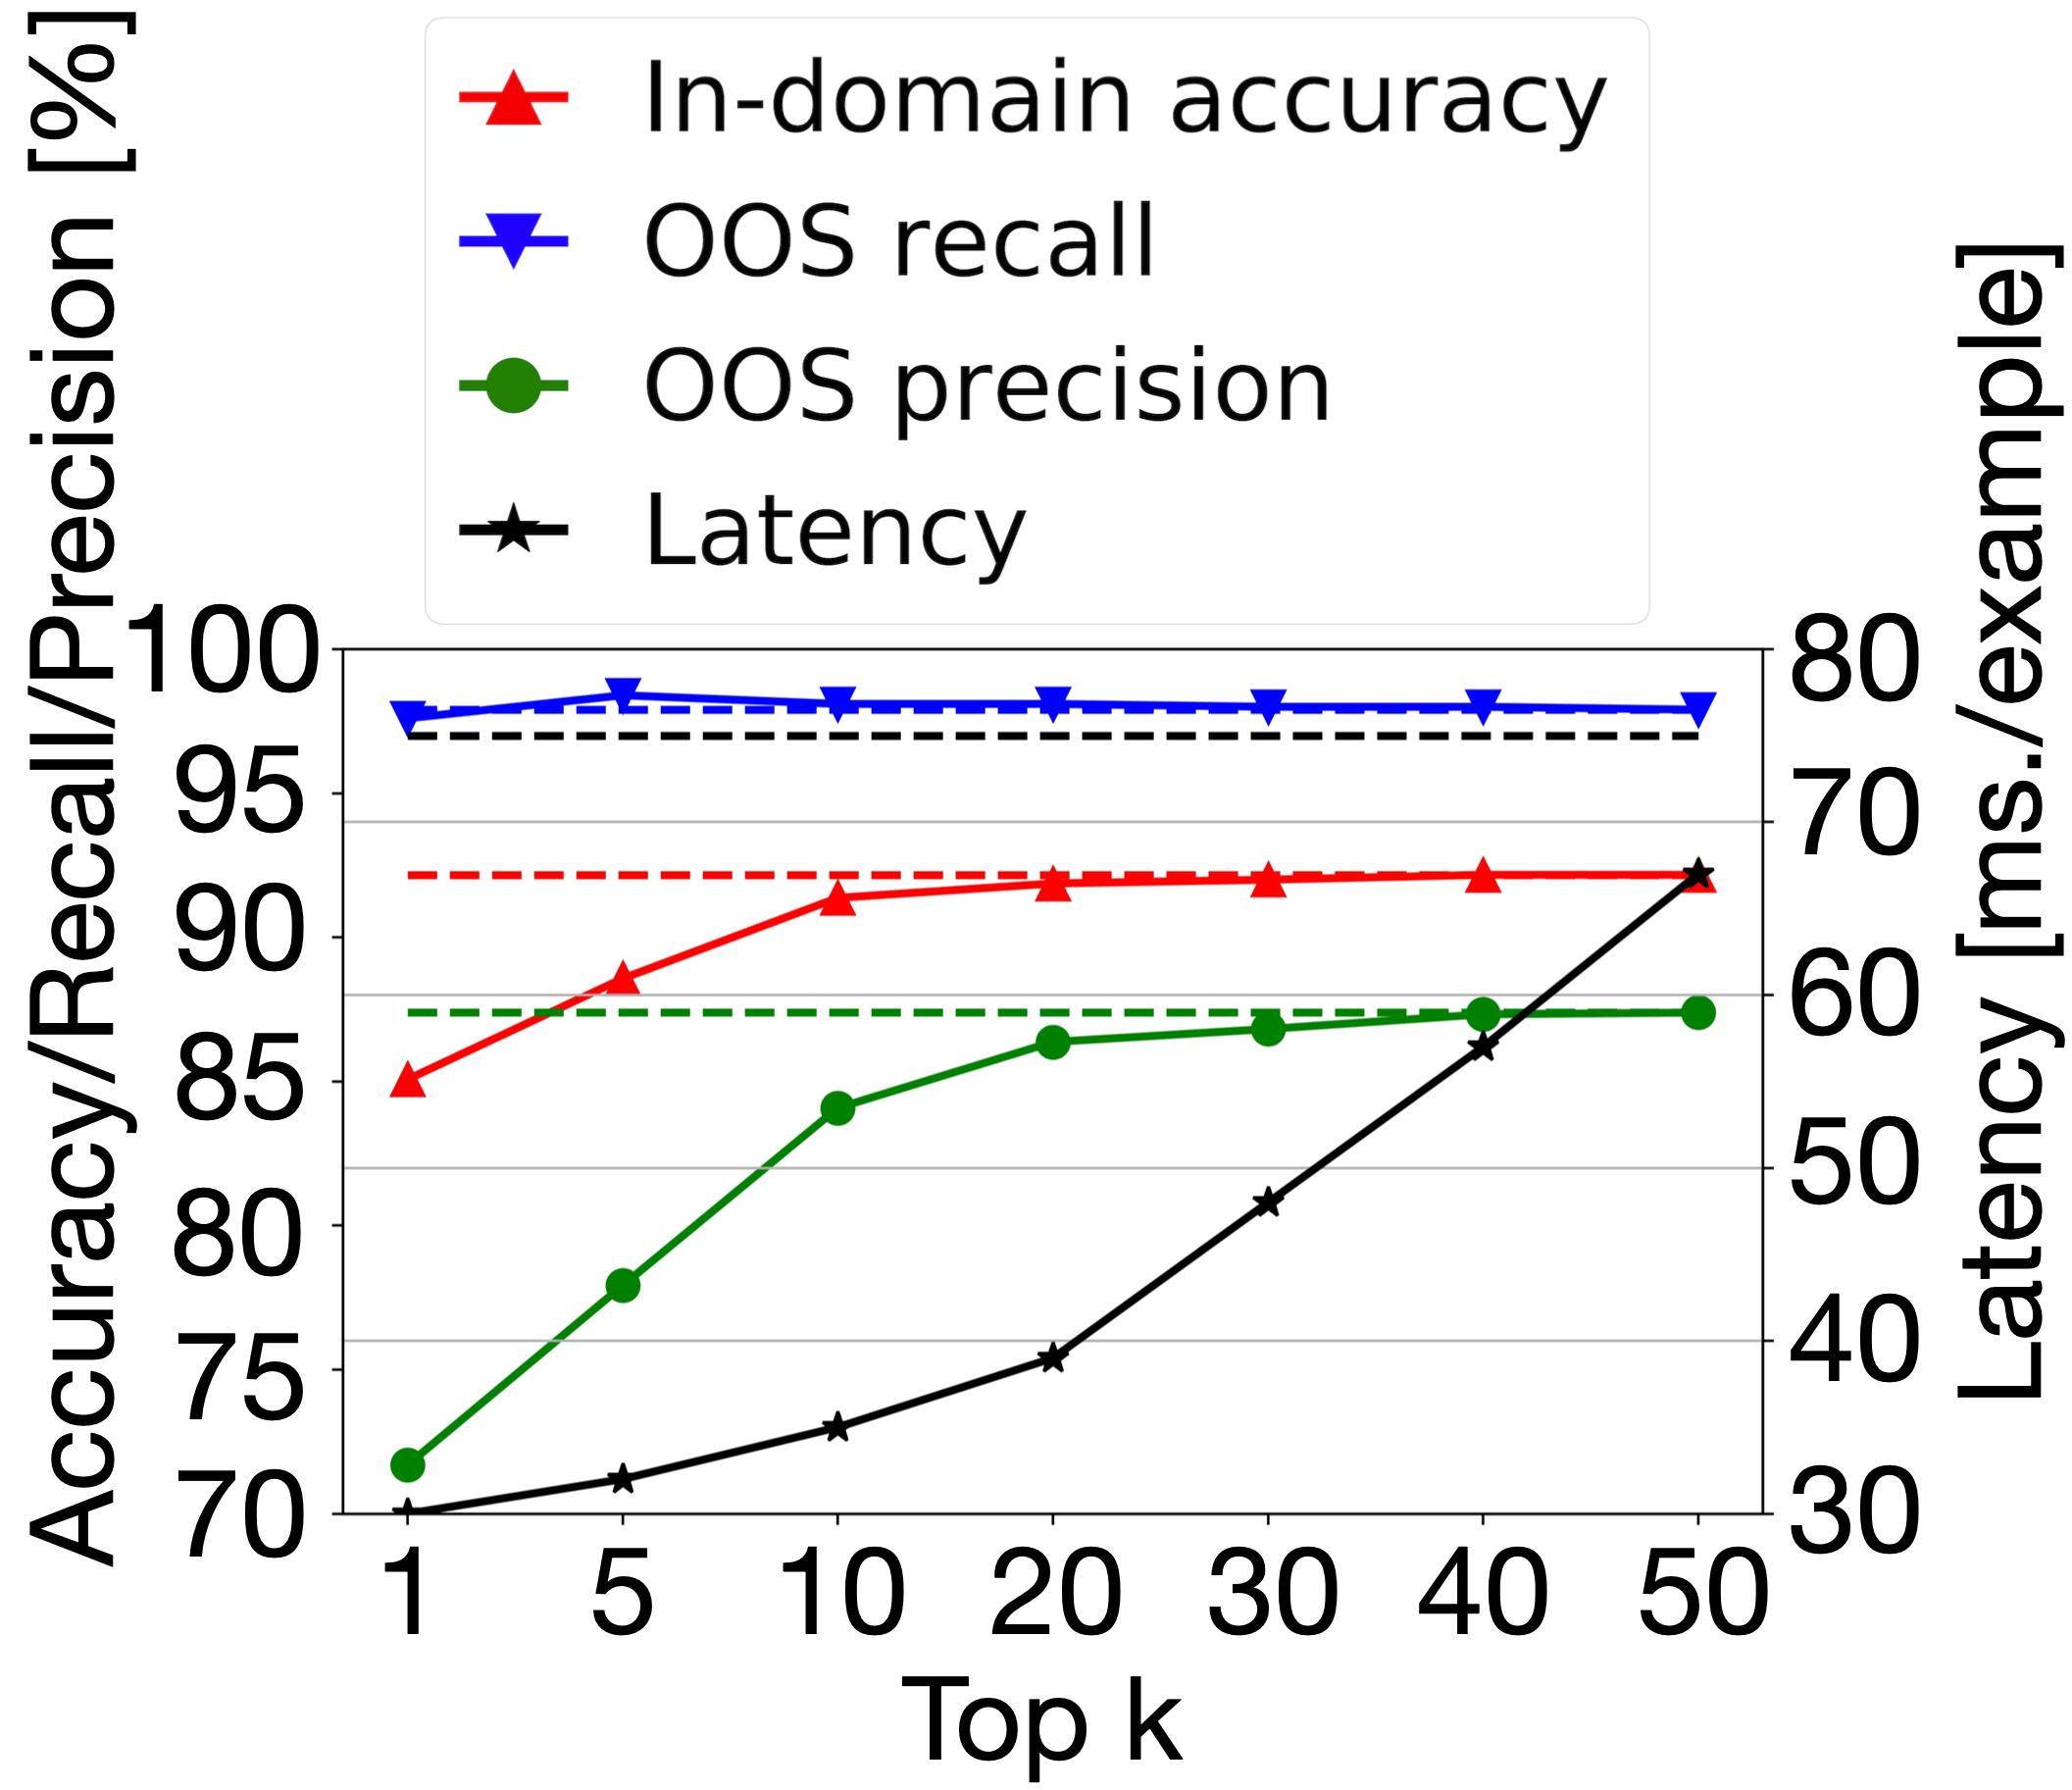
\includegraphics[width=1.\linewidth]{./images/Latency.png}
    \includegraphics[width=1.\linewidth]{./images/latency.png}
    \caption{Accuracy vs. latency of DNNC-joint.}
    \label{fig:join-nli}
\end{minipage}%
%}% 
\centering
%\caption{hello world}
%\vspace{-0.5em}
\label{fig:compare_fig}
\end{figure*}
%%%%%%%%%%%%%%%%%%%%%%%%%%%%%%%%




%%%%%%%%%%%%%%%%%%%%%%%%%%%%%%%%%%
\begin{table*}[]
\centering
\small
\resizebox{1.0\linewidth}{!}{
\begin{tabular}{l|cc|cc|cc|cc|rr}
\hline
                     & \multicolumn{2}{c|}{\textbf{In-domain accuracy}}  & \multicolumn{2}{c|}{\textbf{OOS recall}} & \multicolumn{2}{c|}{\textbf{OOS precision}}       & \multicolumn{2}{c}{\textbf{OOS F1}} & \multicolumn{2}{c}{\textbf{Latency [ms./example]}} \\
\textbf{Banking}              & \textbf{5-shot}                & \textbf{10-shot} & \textbf{5-shot}    & \textbf{10-shot}    & \textbf{5-shot}         & \textbf{10-shot}        & \textbf{5-shot}  & \textbf{10-shot} & \textbf{5-shot}   & \textbf{10-shot}  \\ \hline
TF-IDF-$k$NN               & 59.2 $\pm$ 3.6                 & 65.9 $\pm$ 3.8   & 61.0 $\pm$ 2.8     & 51.3 $\pm$ 1.6      & 97.6 $\pm$ 0.6 & 98.2 $\pm$ 0.3 &      75.1  $\pm$ 2.2           &    67.4 $\pm$ 1.3              & 1                 & 1                 \\
Emb-$k$NN-vanilla           &   64.4 $\pm$ 2.8              &  65.4 $\pm$ 2.3    &  89.5 $\pm$ 1.1   &  94.6 $\pm$ 0.5     &     95.1 $\pm$ 0.5       &  92.6 $\pm$ 0.7       & 92.2 $\pm$ 0.5  & 93.6 $\pm$ 0.5  &     15        & 15           \\
Emb-$k$NN            & 78.4 $\pm$ 2.4                 & 84.3 $\pm$ 1.2   & 92.0 $\pm$ 2.0     & 91.6 $\pm$ 1.2      & 91.4 $\pm$ 0.8          & 93.7 $\pm$ 0.5          & 91.7 $\pm$ 0.7   & 92.6 $\pm$ 0.7   & 15             & 15             \\
RN-$k$NN            &     79.5  $\pm$ 3.1           & 89.0 $\pm$ 1.4    &  88.3 $\pm$ 1.9    &  75.9 $\pm$ 4.0     &    91.6 $\pm$ 1.3       &   95.9 $\pm$ 0.6     &  89.9 $\pm$ 1.0  & 84.7 $\pm$ 2.5 & 17             & 17             \\ \hdashline
DNNC-joint   & 88.5 $\pm$ 1.2                 & 91.0 $\pm$ 1.0   & 95.0 $\pm$ 0.9     & 95.2 $\pm$ 1.1      & 96.9 $\pm$ 0.4          & 97.3 $\pm$ 0.4          & 96.0 $\pm$ 0.5   & 96.3 $\pm$ 0.6   & 36             & 36             \\ 
DNNC        & 88.6 $\pm$ 1.3                 & 91.2 $\pm$ 1.1   & 94.7 $\pm$ 1.0     & 94.8 $\pm$ 1.1      & 97.0 $\pm$ 0.3          & 97.5 $\pm$ 0.4          & 95.9 $\pm$ 0.5   & 96.1 $\pm$ 0.6   & 73             & 143             \\ \hline
%classifier           & 79.7 $\pm$ 1.8                 & 85.2 $\pm$ 1.3   & 93.3 $\pm$ 2.9     & 93.3 $\pm$ 1.0      & 92.5 $\pm$ 0.9          & 94.4 $\pm$ 0.5          & 92.9 $\pm$ 1.8   & 93.8 $\pm$ 0.6   & 26             & 26             \\ \hline
\textbf{All domains} & \textbf{5-shot}                & \textbf{10-shot} & \textbf{5-shot}    & \textbf{10-shot}    & \textbf{5-shot}         & \textbf{10-shot}        & \textbf{5-shot}  & \textbf{10-shot} & \textbf{5-shot}   & \textbf{10-shot}  \\ \hline
TF-IDF-$k$NN               & 35.4 $\pm$ 0.7                 & 31.3 $\pm$ 1.1   & 72.2 $\pm$ 2.1     & 83.1 $\pm$ 1.5      & 24.7 $\pm$ 0.4          & 23.5 $\pm$ 0.4          &     36.8 $\pm$    0.6          &   36.6 $\pm$ 0.6              & 1             & 2             \\
Emb-$k$NN-vanilla           &  54.2 $\pm$ 0.5              &  50.7 $\pm$ 0.9 &   87.5 $\pm$ 0.7  &   95.1 $\pm$ 0.3  &  39.6 $\pm$ 0.3       &  34.2 $\pm$ 0.3    & 54.5 $\pm$ 0.4 & 50.3 $\pm$ 0.3  &   16        &     19         \\
Emb-$k$NN            &         78.7 $\pm$ 1.0                       &     86.9  $\pm$ 0.3            &     86.8 $\pm$ 2.4               &   82.3 $\pm$ 0.8                 &           55.0 $\pm$ 1.5              &      66.5 $\pm$ 1.0                   &        67.3 $\pm$ 1.6          &       73.5 $\pm$ 0.7          &         16          &     19              \\
RN-$k$NN             &    76.6 $\pm$ 0.6      &      88.7  $\pm$ 1.1        &    88.9 $\pm$ 1.4                &     76.6 $\pm$ 2.7               &   50.0 $\pm$ 0.3                       &      71.0 $\pm$ 0.5                  &           64.0   $\pm$ 0.2     &       73.7 $\pm$ 1.0         &     16              &    18               \\ \hdashline
DNNC-joint   & 84.5 $\pm$ 0.8 & 91.2 $\pm$ 0.2   & 90.6 $\pm$ 1.6     & 85.1 $\pm$ 1.8      & 63.6 $\pm$ 2.4          & 78.4 $\pm$ 2.1          &        74.7  $\pm$ 1.9         &     81.6 $\pm$ 0.4             & 37             & 41             \\ 
DNNC        & 84.9 $\pm$ 0.8                 & 91.6 $\pm$ 0.3   & 90.1 $\pm$ 1.6     & 83.0 $\pm$ 2.0      & 64.7 $\pm$ 2.5          & 81.4 $\pm$ 2.0          &            75.3 $\pm$ 2.0       &   82.1 $\pm$ 0.3                        & 697             & 1498             \\ \hline
%classifier           & 77.7 $\pm$ 0.6                 & 83.2 $\pm$ 0.6   & 91.9 $\pm$ 1.1     & 92.9 $\pm$ 0.8      & 53.9 $\pm$ 0.8          & 58.2 $\pm$ 1.0          & 68.0 $\pm$ 1.0   & 71.6 $\pm$ 0.8   & 26            & 26            \\ \hline
\end{tabular}}\caption{Comparison among the nearest neighbor methods on the test sets for the banking domain and all the domains. The latency is measured on a single NVIDIA Tesla V100 GPU, where the batch size is $1$ to simulate an online use case. DNNC-joint is based on top-20 Emb-$k$NN retrieval. }
\label{table:latency}
%\vspace{-0.5em}
\end{table*}
%%%%%%%%%%%%%%%%%%%%%%%%%%%%%%%%%%%%%%%



%%%%%%%%%%%%%%%%%%%%%%%%%%%%%%%%%%%%%%%%%%%%%%%%%%
% \begin{table*}[]
% \centering
% \small
% \resizebox{0.8\linewidth}{!}{
% \begin{tabular}{l|cc|cc|cc}
% \hline
%                           & \multicolumn{2}{c|}{\textbf{In-Domain accuracy}}      & \multicolumn{2}{c|}{\textbf{OOS recall}}      & \multicolumn{2}{c}{\textbf{OOS precision}}   \\
%                           & \textbf{5-Shot}           & \textbf{10-Shot}          & \textbf{5-Shot}            & \textbf{10-Shot}          & \textbf{5-Shot}           & \textbf{10-Shot}          \\ \hline
% classifier                & 77.4 $\pm$ 2.5         & 74.3 $\pm$ 2.6          & 75.7 $\pm$ 6.6           & 79.9 $\pm$ 9.2         & 64.3 $\pm$ 3.4          & 62.0 $\pm$ 2.3        \\
% nli-Fine-Tune             & 72.9 $\pm$ 5.7          & 88.9 $\pm$ 1.7          & 80.1 $\pm$ 11.9         & 52.9 $\pm$ 8.5          & 61.9 $\pm$ 3.7          & 78.3 $\pm$ 4.8          \\ \hdashline
% classifier (OOS-train)    & \textbf{88.4 $\pm$ 2.4} & \textbf{90.6 $\pm$ 2.3} & 42.3 $\pm$ 12.0         & 60.8 $\pm$ 7.3          & \textbf{88.2 $\pm$ 7.4} & \textbf{93.6 $\pm$ 4.5} \\
% nli-Fine-Tune (OOS-train) & 80.6 $\pm$ 3.1        & 87.3 $\pm$ 2.0          & \textbf{81.2 $\pm$ 10.2} & \textbf{80.7 $\pm$ 6.7} & 70.8$\pm$ 3.6          & 81.3 $\pm$ 3.6          \\ \hline
% \end{tabular}}\caption{Testing results on the specific banking domain.}
% \end{table*}


% \begin{figure*}%[H]
%     %\fbox{\rule{0pt}{3.0 in}
%     %\centering
%     \begin{center}
%     \includegraphics[width=1\linewidth]{./images/5-10-shot-Visualization_flat.jpg}
%     \end{center}
%     %\rule{.9\linewidth}{0pt}}
%     \caption{5-shot and 10-shot validation results on the banking domain. In this series of plots, a model with a higher area-under-the-curve is more robust.}
%     \label{fig:merged-figures}
%     %\vspace{-1em}
% \end{figure*}


\subsection{Robustness of DNNC}
As described in Section~\ref{subsection:evalMetrics}, we select the threshold to determine OOS by making a trade-off between in-domain classification and OOS detection accuracy.
It is therefore desirable to have a model with candidate thresholds that provide high in-domain accuracy as well as OOS precision and recall. 
\if0
We observe in Figure~\ref{fig:robust} that in the 5-shot setting, in-domain accuracy and OOS detection precision for both DNNC-scratch and classifier models drop rapidly as the threshold increases, while the OOS recall increases rapidly with the threshold. In contrast, the DNNC demonstrates robust performances across all three metrics with the changes in the threshold. \fi


%In the case of 10-shot (right column of Figure~\ref{fig:robust}), while all three methods improve across the three metrics under consideration and the gap between NLI-Fine-Tune and the other two on in-domain accuracy shrinks, the NLI-Fine-Tune method remains dominant and significantly more robust on the OOS detection task.

We observe in Figure~\ref{fig:robust} that in the 5-shot setting, DNNC is the most robust to the threshold selection.
The contrast between the classification model and DNNC-scratch suggests that nearest neighbor approaches (in this case DNNC) make for stronger discriminators; the advantage of DNNC over DNNC-scratch further demonstrates the power of the NLI transfer and, perhaps more importantly, the effectiveness of the pairwise discriminative pre-training.
This result is consistent with the intuition we gained from Figure~\ref{fig:tsne-main}, and the overall observation is also consistent across different settings.

% \begin{figure*}%[H]
%     %\fbox{\rule{0pt}{3.0 in}
%     %\centering
%     \begin{center}
%     \includegraphics[width=1\linewidth]{./images/5-10-shot-Visualization_flat.jpg}
%     \end{center}
%     %\rule{.9\linewidth}{0pt}}
%     \caption{5-shot and 10-shot validation results on the banking domain. In this series of plots, a model with a higher area-under-the-curve is more robust.}
%     \label{fig:robust}
%     %\vspace{-1em}
% \end{figure*}

To further understand the differences in behaviors between the classification model and DNNC method, we examine the output from the final softmax/sigmoid function (model confidence score) in Figure~\ref{fig:separation}.
At 5-shot, the classifier method still struggles to fully distinguish the in-domain examples from the OOS examples in its confidence scoring, while DNNC already attains a clear distinction between the two.
Again, we can clearly see the effectiveness of the NLI transfer.

With the model architectures for BERT-based classifier and DNNC being the same (RoBERTa is used for both methods) except for the final layer (multi-class-softmax vs. binary sigmoid), this result suggests that the pairwise NLI-like training is more sample-efficient, making it an excellent candidate for the few-shot use case.

% \begin{figure*}%[H]
%     %\fbox{\rule{0pt}{3.0 in}
%     %\resizebox{1.0\linewidth}{!}{%
%     %\centering
%     \begin{center}
%     \includegraphics[width=1.0\textwidth]{./images/5-10-shot-Conf-flat.jpg}%}
%     \end{center}
%     %\rule{.9\linewidth}{0pt}}
%     \caption{5-shot and 10-shot testing results on the banking domain and all domains.}
%     \label{fig:separation}
%     %\vspace{-1em}
% \end{figure*}

\subsection{DNNC-joint for Faster Inference}
Despite its effectiveness in few-shot intent and OOS settings, the proposed DNNC method might not scale in high-traffic use cases, especially when the number of classes, $N$, is large, due to the inference-time bottleneck (Section~\ref{subsec:joint}).
With this in mind, we proposed the DNNC-joint approach, wherein a faster model is used to filter candidates for the fine-tuned DNNC model. 

We compare the accuracy and inference latency metrics for various methods in Table~\ref{table:latency}.
Note that Emb-$k$NN and RN-$k$NN exhibit excellent latency performance, but they fall considerably short in both the in-domain intent and OOS detection accuracy, compared to DNNC and the DNNC-joint methods.
On the other hand, the DNNC-joint model shows competitiveness in both inference latency and accuracy.
These results indicate that the current text embedding approaches like SBERT are not enough to fully capture fine-grained semantics.
%(36ms/example in latency, 88.5\% in-domain accuracy at 5-shot). 

Intuitively, there is a trade-off between latency and inference accuracy: with aggressive filtering, the DNNC inference step needs to handle a smaller number of training examples, but might miss informative examples; with less aggressive filtering, the NLI model sees more training examples during inference, but will take longer to process single user input.
This is illustrated in Figure~\ref{fig:join-nli}, where the in-domain intent and OOS accuracy metrics (on the development set of the banking domain in the 5-shot setting) improve with the increase of $k$, while the latency increases at the same time.
Empirically, $k=20$ appears to strike the balance between latency and accuracy, with the accuracy metrics similar to those of the DNNC method, while being much faster than DNNC (dashed lines are the corresponding DNNC references).



% \begin{figure}%[H]
%     %\fbox{\rule{0pt}{3.0 in}
%     \centering
%     \resizebox{1.0\linewidth}{!}{%
%     \centering
%     \includegraphics[width=1.0\textwidth]{./images/5-10-shot-Joint_NLI.jpg}}
%     %\rule{.9\linewidth}{0pt}}
%     \caption{5-shot and 10-shot joint-nli results on the banking domain. Where the dash lines are nli-fine-tune results}
%     \label{fig:join-nli}
%     %\vspace{-1em}
% \end{figure}

%%%%% Temporarily remove this
\if0
\subsection{Training with OOS examples}

\paragraph{OOS examples}
We could optionally have access to training examples of the OOS utterances, so that the model can explicitly learn to detect OOS utterances.
In this case we also have $K$ training examples: $(e'_1, e'_2, \ldots, e'_K)$.
It should be noted that arbitrary utterances can be the OOS examples which are {\it not} categorized into any of the $N$ intent classes, and the definition of OOS is different depending on $\mathbf{C}$.
It is thus ideal not to assume the access to enough amount of the OOS examples, from the viewpoint of out-of-distribution detection.

\paragraph{OOS as an extra class:}
The second strategy is to add an extra class for OOS to formulate an $(N+1)$-class classification task.
This is possible {\it only} when we have the OOS training examples.
At inference time, we do not need to set the threshold because OOS is treated as one of the classes.

\paragraph{Training with OOS examples}
We can add more negative examples when the OOS training examples are available.
The objective of using the OOS examples is to help the model explicitly learn to reject the OOS examples based on the in-domain examples.
We therefore create such pairs: $(e'_{\ell}, e_{j, i})$, whereas we do not consider $(e_{j, i}, e'_{\ell})$.
In total, we have $NK^2$ additional negative examples.
The example (c) in Table~\ref{tb:examples} shows that the request in the input sentence is not supported in the dataset, and thus does not match the other sentence's intent.\footnote{Another alternative strategy is to use $N$ binary classifiers as in one-vs.-rest classification, instead of the softmax classifier in Equation~(\ref{eq:softmax}).
This is also attractive in that we can unify the two strategies.
However, we did not observe empirical advantage above the softmax classifier.}
\fi